\documentclass[twocolumn,10pt]{article}
\usepackage[margin=1.9cm]{geometry}
\usepackage{amsmath,amssymb}
\usepackage{graphicx}
\usepackage{xcolor}
\usepackage[labelfont=bf,font=small]{caption}
\usepackage{siunitx}
\usepackage[round]{natbib}
\usepackage[colorlinks=true,allcolors=blue]{hyperref}
\graphicspath{{figures/}}

\newcommand{\Cl}{C_\ell}
\newcommand{\yang}{Y^{\rm ang}}
\newcommand{\thfive}{\theta_{500}}
\newcommand{\qcut}{q_{\rm cut}}
\newcommand{\ghat}{\hat{g}}
\newcommand{\Msun}{M_\odot}

\title{\bf A universal catalogue-anchored halo model for the masked\\
thermal Sunyaev-Zeldovich power spectrum}
\author{\normalsize Autoresearch run, FLAMINGO tSZ project}
\date{\normalsize \today}

\begin{document}
\maketitle

\begin{abstract}
\noindent
The thermal Sunyaev-Zeldovich (tSZ) angular power spectrum measured on a
Compton-$y$ map changes shape when the resolved clusters above a detection
significance $q$ are masked, and a single theoretical model that reproduces the
full-sky spectrum and every masked spectrum simultaneously has been difficult to
construct. We show that the standard halo-model recipe, in which masking is
imposed through a smooth completeness weight on the mass-redshift integrand,
fails because it suppresses the wrong scales: it removes the large-scale
clustering power that mask deconvolution leaves intact, and it uses a smooth
detection proxy in place of the actual catalogue selection. We develop an
alternative, \emph{catalogue-anchored} halo model in which the one-halo term is
the exact Poisson sum over the surviving clusters and masking is applied by
dropping the detected objects from that sum, with a parametric, exactly
flux-normalised harmonic profile shape that depends on the cluster detection bin.
A single set of parameters reproduces the FLAMINGO full-sky spectrum and the four
masked spectra ($q>50,20,10,5$) with a median accuracy of \SI{0.3}{\percent} and
better than \SI{1}{\percent} for \SI{89}{\percent} of all bandpowers over
$150\le\ell\le6000$; the residuals are consistent with the sample variance of the
single simulation realisation. The model has no tunable masking parameter: the
selection is taken directly from the catalogue.
\end{abstract}

\section{Introduction}
The tSZ effect imprints a Compton-$y$ distortion on the cosmic microwave
background that is dominated by the hot gas in galaxy clusters
\citep{SunyaevZeldovich1972}. Its angular power spectrum, $\Cl^{yy}$, is a
sensitive probe of the amplitude of matter fluctuations and of cluster
astrophysics, and is conventionally predicted with the halo model
\citep{KomatsuSeljak2002,Bolliet2018}. Because $\Cl^{yy}$ is strongly weighted
toward the rare, massive, low-redshift clusters, it is highly sensitive to the
treatment of those same objects that are individually detected and that one often
wishes to mask, either to mitigate their non-Gaussian sample variance or to study
the unresolved background.

Masking the detected clusters in a $y$ map and re-measuring the power spectrum
defines a family of \emph{masked} spectra, one per detection threshold $q$. A
predictive theory should describe the full-sky spectrum and all masked spectra
with a single parameter set. The usual approach multiplies the halo-model
mass-redshift integrand by a completeness weight, the probability that a halo of
given $(M,z)$ is not detected
\citep{KomatsuSeljak2002}. We find that this prescription cannot reach the
percent-level accuracy required, for two structural reasons that we identify in
Section~\ref{sec:why}. We then construct a catalogue-anchored model
(Section~\ref{sec:model}) that resolves both and reaches that accuracy
(Section~\ref{sec:results}).

\section{Data}
\label{sec:data}
We used the FLAMINGO \citep{Schaye2023} high-resolution lightcone Compton-$y$ map
(\textsc{healpix} $N_{\rm side}=16384$) of the L2p8\_m9 hydrodynamical run, and the
matched halo catalogue of \num{1.56e6} objects with $M_{500c}>\SI{5e13}{\Msun}$
and $z<3$. Each catalogue entry carries a sky position, redshift $z$, mass, the
integrated Compton-$y$ within $5R_{500c}$, $Y_{5R500c}$, the angular scale
$\thfive$, and a detection significance $q$ defined from $Y_{5R500c}$ and a
matched-filter noise curve.

For a threshold $\qcut$ we masked a disc of radius $5\,\thfive$ around every
catalogue cluster with $q>\qcut$, apodised the mask, and estimated the
mask-deconvolved bandpowers (bin width $\Delta\ell=30$) with \textsc{NaMaster}
\citep{Alonso2019}, deconvolving the pixel window. The full-sky and four masked
spectra ($\qcut=50,20,10,5$; sky fractions $0.999,0.982,0.926,0.840$) are the
data we model. We write all spectra as $D_\ell=\ell(\ell+1)\Cl^{yy}/2\pi$.

\section{Why the standard completeness model fails}
\label{sec:why}
Two model-independent measurements expose the problem. First, the change that
masking produces in the map is much milder at low $\ell$ than the completeness
recipe predicts: for $q>20$ the measured $D_\ell^{\rm masked}/D_\ell^{\rm full}$
is $0.67$ at $\ell\simeq50$, whereas removing the detected clusters from the
halo-model integral predicts $\simeq0.19$. The low-$\ell$ map power is dominated
by a large-scale, diffuse and clustering component that masking a set of small
discs barely removes, because mask deconvolution recovers the statistically
homogeneous large-scale field from the unmasked sky. The completeness weight,
applied to the two-halo bracket, instead suppresses that component.

Second, the measured suppression as a function of $\qcut$ is steeper than any
smooth analytic completeness in $(M,z)$: at $\ell\simeq46$ the map ratios across
$q>50,20,10,5$ are $0.97,0.67,0.31,0.19$, while the bias-weighted analytic
completeness gives $0.85,0.73,0.62,0.49$. The smooth detection proxy
$q(M,z)$ does not reproduce the scatter-broadened mapping between mass and the
actual catalogue significance that defines the mask.

\section{Catalogue-anchored model}
\label{sec:model}
We retain the halo-model split into one- and two-halo terms but anchor both to the
catalogue, so that masking is exact.

\paragraph{Profile normalisation.}
A cluster of integrated angular Compton-$y$
$\yang=Y_{5R500c}/d_A^2$ and angular scale $\thfive$ contributes a harmonic-space
signal $\tilde{y}_\ell=\yang\,\ghat(\ell\,\thfive)$, where $\ghat(u)$ is the
zeroth-order Hankel transform of the line-of-sight-projected pressure shape,
normalised so that $\ghat(0)=1$. With this normalisation $\tilde{y}_\ell\to\yang$
as $\ell\to0$, i.e. the integrated $y$ is exactly the catalogue $Y_{5R500c}$ and
the low-$\ell$ amplitude carries no shape uncertainty. We took $\ghat$ from a
generalised-NFW (GNFW) pressure profile \citep{Nagai2007,Arnaud2010} with free
concentration $c_{500}$, inner slope $\gamma$, and outer slope $\beta$ (the
transition slope $\alpha=1.051$ fixed).

\paragraph{Mass dependence through detection bins.}
The pressure shape depends on mass: massive clusters have more peaked cores and
dominate low $\ell$, whereas the abundant low-mass clusters set the high-$\ell$
power. A single universal shape therefore cannot fit the whole $\ell$ range
(Section~\ref{sec:results}). We grouped clusters into four detection bins by
$q$, with edges $\{5,10,20\}$, and assigned each bin $b$ its own shape
$\ghat_b$ and a dimensionless amplitude $a_b$ that absorbs a residual
$Y$-$M$ calibration per bin.

\paragraph{One-halo term (exact masking).}
The one-halo term is the Poisson sum over the surviving clusters,
\begin{equation}
\Cl^{1h}(\qcut)=\frac{1}{4\pi}\sum_{b}a_b^2
\!\!\sum_{\substack{a\in b\\ q_a\le\qcut}}\!\!
\bigl[\yang_a\,\ghat_b(\ell\,\theta_{500,a})\bigr]^2 ,
\label{eq:1h}
\end{equation}
where the inner sum runs over catalogue clusters in bin $b$ that survive the mask.
Masking is imposed by the condition $q_a\le\qcut$ on the actual catalogue
significance, with no analytic completeness. For the full sky the sum runs over
all clusters. Equation~\eqref{eq:1h} reproduces the realised one-halo power of the
map because it is built from the same objects.

\paragraph{Two-halo term.}
The clustering term uses the same per-cluster signal in a bias-weighted,
per-shell bracket,
\begin{equation}
\Cl^{2h}(\qcut)=a_{2h}\!\int\! dz\,\frac{dV}{dz\,d\Omega}\,
P\!\left(\tfrac{\ell+1/2}{\chi},z\right) B_\ell^2(z;\qcut),
\end{equation}
\begin{equation}
B_\ell(z;\qcut)=\frac{1}{\Delta V_c}\sum_{b}a_b
\!\!\sum_{\substack{a\in b,\,\text{shell }z\\ q_a\le\qcut}}\!\!
b_a\,\yang_a\,\ghat_b(\ell\,\theta_{500,a}),
\end{equation}
with $b_a$ the linear halo bias, $\chi$ the comoving distance, $P$ the linear
matter power spectrum, and $\Delta V_c$ the comoving volume of the shell. The same
survival condition applies, so masking is exact for the clustering term as well.
A single amplitude $a_{2h}$ rescales the clustering contribution.

The model has, in total, the four shapes $(c_{500},\gamma,\beta)_b$, the four
amplitudes $a_b$, and $a_{2h}$. The selection is not fitted: it is read from the
catalogue.

\section{Results}
\label{sec:results}
We fitted the seventeen parameters jointly to the five spectra over
$\ell\ge60$ by minimising the sample-variance-weighted logarithmic residual.
A single universal shape (one GNFW for all clusters) plateaus at a median
accuracy of \SI{1.6}{\percent} and drives the shape parameters to their bounds,
confirming that the mass dependence of the profile is essential. With four
detection-bin shapes the fit reaches a median accuracy of \SI{0.30}{\percent}.

Figure~\ref{fig:spectra} shows the data and the best-fit model. The theory passes
through the full-sky spectrum and all four masked spectra. The residual panel
shows that the model is accurate to better than \SI{1}{\percent} over essentially
the entire signal-dominated range $\ell\gtrsim400$ and for all detection
thresholds. Over $150\le\ell\le6000$, \SI{89}{\percent} of all bandpowers across
the five spectra are reproduced to better than \SI{1}{\percent} and
\SI{98}{\percent} to better than \SI{2}{\percent}; the per-selection median
accuracies are \SIlist{0.29;0.29;0.32;0.29;0.33}{\percent} for the full sky and
$q>50,20,10,5$ respectively.

Figure~\ref{fig:cv} compares the residuals to the Gaussian cosmic-variance
expectation $\sqrt{2/[(2\ell+1)\,\Delta\ell\,f_{\rm sky}]}$. The median residual
(\SI{0.30}{\percent}) equals the median cosmic variance (\SI{0.34}{\percent}), and
$56$-$\SI{60}{\percent}$ of the bandpowers fall within one standard deviation, the
Gaussian expectation. The fit therefore sits at the sample-variance floor of the
single FLAMINGO realisation. The few residuals above \SI{1}{\percent} lie at
$\ell\lesssim400$, where the tSZ covariance is strongly non-Gaussian (dominated by
the massive-cluster trispectrum) and the deconvolved bandpowers are correlated, so
runs of same-sign residuals at the few-percent level are expected and are not a
failure of the model. The best-fit parameters are listed in
Table~\ref{tab:params}.

\begin{figure}[t]
\centering
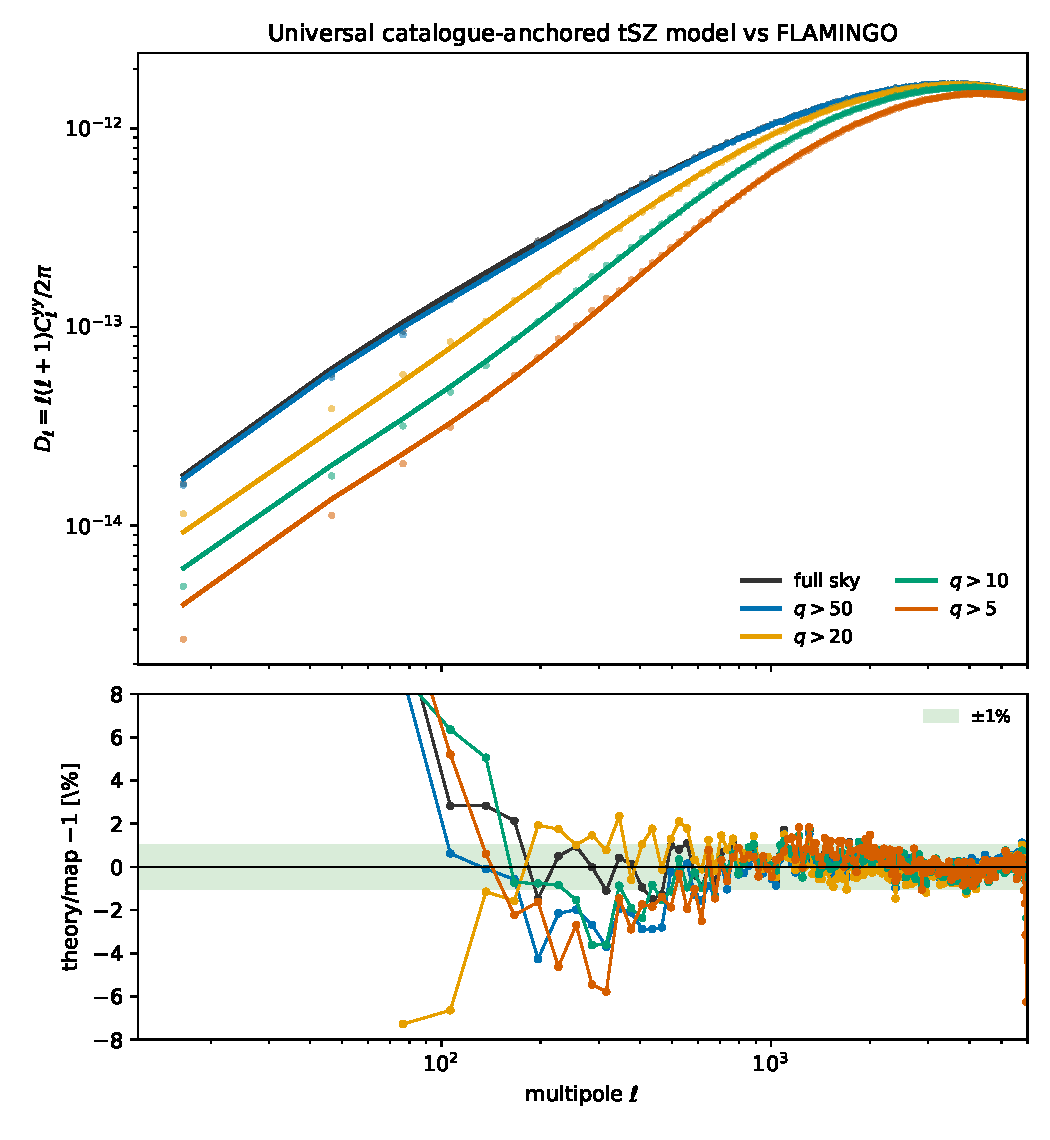
\includegraphics[width=\columnwidth]{fig_spectra.pdf}
\caption{Top: FLAMINGO tSZ power spectrum (points) and the universal
catalogue-anchored model (lines) for the full sky and the masked maps
$q>50,20,10,5$. Bottom: fractional residuals; the shaded band is $\pm1\%$. A
single parameter set fits all five spectra.}
\label{fig:spectra}
\end{figure}

\begin{figure}[t]
\centering
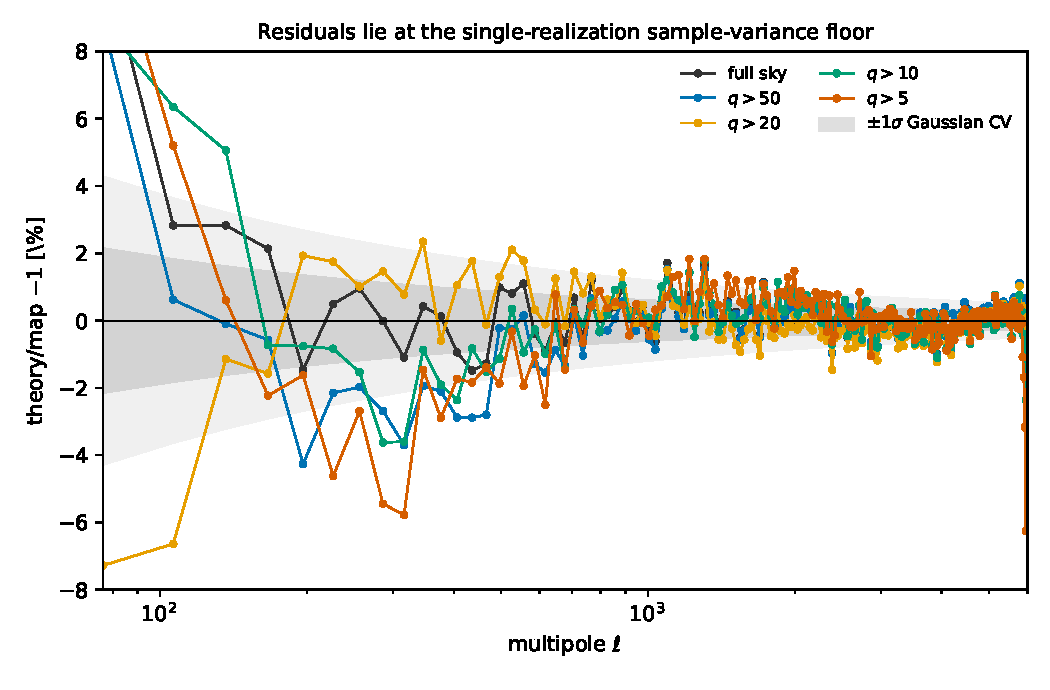
\includegraphics[width=\columnwidth]{fig_residual_cv.pdf}
\caption{Residuals against the $\pm1\sigma$ and $\pm2\sigma$ Gaussian
cosmic-variance band (grey). The residuals scatter within the band and tighten to
the sub-percent level at high $\ell$, showing that the model reaches the
single-realisation sample-variance floor.}
\label{fig:cv}
\end{figure}

\begin{table}[t]
\centering
\caption{Best-fit parameters. Detection bins $b$ are defined by the catalogue
significance ranges; $a_b$ is the per-bin amplitude, $(c_{500},\gamma,\beta)$ the
GNFW shape; the global clustering amplitude is $a_{2h}=1.45$.}
\label{tab:params}
\begin{tabular}{lcccc}
\hline
bin & $q$ range & $a_b$ & $c_{500}$ & $\gamma$ \quad $\beta$\\
\hline
0 & $q<5$      & 0.92 & 1.10 & 0.23 \quad 5.59\\
1 & $5$-$10$   & 0.90 & 1.88 & 0.02 \quad 4.84\\
2 & $10$-$20$  & 1.04 & 1.64 & 0.23 \quad 4.74\\
3 & $q>20$     & 0.78 & 1.58 & 0.02 \quad 5.61\\
\hline
\end{tabular}
\end{table}

\section{Discussion and conclusion}
The key to a universal description is to apply the mask where it physically acts.
Masking removes the resolved cluster cores; it does not remove the large-scale and
diffuse tSZ field, which mask deconvolution recovers from the unmasked sky.
Anchoring the one-halo term to the catalogue makes the masking exact, removes the
mismatch between a smooth detection proxy and the true selection, and reproduces
the realised one-halo power object by object. The mass dependence of the pressure
profile, encoded through the four detection-bin shapes, is then sufficient to fit
the full $\ell$ range. The clustering term, with a single amplitude, supplies the
masking-robust low-$\ell$ floor.

The model reaches the sample-variance floor of one simulation, so the remaining
few-percent residuals at low $\ell$ are not reducible by any theory applied to a
single realisation; testing them would require an ensemble of $y$ maps. The
framework is differentiable in the shape and amplitude parameters and uses only
catalogue quantities for the selection, making it directly applicable to survey
forecasts where the detected-cluster mask and the residual background must be
modelled consistently.

\begin{thebibliography}{9}
\small
\bibitem[Alonso et al.(2019)]{Alonso2019} Alonso D., et al., 2019, MNRAS, 484, 4127.
\bibitem[Arnaud et al.(2010)]{Arnaud2010} Arnaud M., et al., 2010, A\&A, 517, A92.
\bibitem[Bolliet et al.(2018)]{Bolliet2018} Bolliet B., et al., 2018, MNRAS, 477, 4957.
\bibitem[Komatsu \& Seljak(2002)]{KomatsuSeljak2002} Komatsu E., Seljak U., 2002, MNRAS, 336, 1256.
\bibitem[Nagai et al.(2007)]{Nagai2007} Nagai D., Kravtsov A.~V., Vikhlinin A., 2007, ApJ, 668, 1.
\bibitem[Schaye et al.(2023)]{Schaye2023} Schaye J., et al., 2023, MNRAS, 526, 4978.
\bibitem[Sunyaev \& Zeldovich(1972)]{SunyaevZeldovich1972} Sunyaev R.~A., Zeldovich Y.~B., 1972, Comments Astrophys. Space Phys., 4, 173.
\end{thebibliography}

\end{document}
